% THIS IS SIGPROC-SP.TEX - VERSION 3.1
% WORKS WITH V3.2SP OF ACM_PROC_ARTICLE-SP.CLS
% APRIL 2009
%
% It is an example file showing how to use the 'acm_proc_article-sp.cls' V3.2SP
% LaTeX2e document class file for Conference Proceedings submissions.
% ----------------------------------------------------------------------------------------------------------------
% This .tex file (and associated .cls V3.2SP) *DOES NOT* produce:
%       1) The Permission Statement
%       2) The Conference (location) Info information
%       3) The Copyright Line with ACM data
%       4) Page numbering
% ---------------------------------------------------------------------------------------------------------------
% It is an example which *does* use the .bib file (from which the .bbl file
% is produced).
% REMEMBER HOWEVER: After having produced the .bbl file,
% and prior to final submission,
% you need to 'insert'  your .bbl file into your source .tex file so as to provide
% ONE 'self-contained' source file.
%
% Questions regarding SIGS should be sent to
% Adrienne Griscti ---> griscti@acm.org
%
% Questions/suggestions regarding the guidelines, .tex and .cls files, etc. to
% Gerald Murray ---> murray@hq.acm.org
%
% For tracking purposes - this is V3.1SP - APRIL 2009

\documentclass{acm_proc_article-sp}

\begin{document}

\title{Comparing and Collaborating Classifiers for Multiclass Image Classification}

%
% You need the command \numberofauthors to handle the 'placement
% and alignment' of the authors beneath the title.
%
% For aesthetic reasons, we recommend 'three authors at a time'
% i.e. three 'name/affiliation blocks' be placed beneath the title.
%
% NOTE: You are NOT restricted in how many 'rows' of
% "name/affiliations" may appear. We just ask that you restrict
% the number of 'columns' to three.
%
% Because of the available 'opening page real-estate'
% we ask you to refrain from putting more than six authors
% (two rows with three columns) beneath the article title.
% More than six makes the first-page appear very cluttered indeed.
%
% Use the \alignauthor commands to handle the names
% and affiliations for an 'aesthetic maximum' of six authors.
% Add names, affiliations, addresses for
% the seventh etc. author(s) as the argument for the
% \additionalauthors command.
% These 'additional authors' will be output/set for you
% without further effort on your part as the last section in
% the body of your article BEFORE References or any Appendices.

\numberofauthors{2} %  in this sample file, there are a *total*
% of EIGHT authors. SIX appear on the 'first-page' (for formatting
% reasons) and the remaining two appear in the \additionalauthors section.
%
\author{
% You can go ahead and credit any number of authors here,
% e.g. one 'row of three' or two rows (consisting of one row of three
% and a second row of one, two or three).
%
% The command \alignauthor (no curly braces needed) should
% precede each author name, affiliation/snail-mail address and
% e-mail address. Additionally, tag each line of
% affiliation/address with \affaddr, and tag the
% e-mail address with \email.
%
% 1st. author
\alignauthor
San-Chuan Hung\\
       \email{sanchuah@andrew.cmu.edu}
% 2nd. author
\alignauthor
Jiajun Wang\\
       \email{jiajunwa@andrew.cmu.edu}
}
\date{30 July 1999}
% Just remember to make sure that the TOTAL number of authors
% is the number that will appear on the first page PLUS the
% number that will appear in the \additionalauthors section.

\maketitle
\begin{abstract}
Many image object recognition methods need machine learning models as the basic training algorithm. In this project we compared the performance four well known machine learning models: Neural Network, Random Forest, Multinomial Logistic Regression, and Support Vector Machine. Furthermore, we analyzed the accuracy of different labels in each classifier, and found that each classifier has its strong points and weak points. We showed that ensemble methods, aggregating different model prediction results, can improve the performance from 0.76\% to 13.07\%.

\end{abstract}

\section{Introduction}
Multiclass Image Classification is to classify images based on image data to multiple classes. Given the pixel values in RGB channels of an image, the machine has to discriminate the image as  a bird, a cat, or a truck. To solve this problem, a common approach is developing multiple computer vision decriptors to help machines to learn how to discriminate different objects, like SIFT \cite{Lowe:2004uq}, and feed the image features into a machine learning algorithm to learn a classifier. 
In this approach, because no matter what kind of image features are developed, it still needs a machine learning classifier in the final step. Machine learning algorithms are important basement. 

In this paper, we mainly compared 4 well-known classification algorithms: Neural Network \cite{HechtNielsen:1989et}, Random Forest\cite{Breiman:2001fb}, Multinomial Logistic Regression\cite{Hosmer:2000vg}, and Support Vector Machine\cite{Vapnik:2000te}. First, we systematically tuned each classifier parameters to its best performance. Second, we compared and analyzed their prediction results: What is the best classifier for the tasks? What are strong labels and weak labels for each classifier?  Last, we came up an ensemble method to aggregate prediction results from different classifiers. 


\section{Background}
\subsection{Multinomial Logistic Regression}
Multinomial Logistic Regression (MLR)\cite{Hosmer:2000vg} is a machine learning model extending Logistic Regression from binary class classification to multi-class classification. Similar to Logistic Regression, MLR learns a vector of linear model parameters $W_k$ of $X$ for each label $k$, and uses sigmoid function to generate the probability of each label. We used the implementation of MLR in provided matlab code, and tuned the parameter of cost and the gamma value of RBF kernel.

\subsection{Support Vector Machine}
Support Vector Machine(SVM)\cite{Vapnik:2000te} is a machine learning model to find a boundary to maximize the gap between different class instances. We used the implementation of SVM in provided matlab code, and tuned the parameter of cost and the gamma value of RBF kernel.

\subsection{Radial Basis Function Kernel}
Radial Basis Function Kernel(RBF Kernel)\cite{Perner:2001wu} is a kernel trick to convert origin feature samples into input space where . We used the implementation of provided matlab code, and tuned the parameter of gamma.

\subsection{Multilayer Neural Network}
Neural network \cite{HechtNielsen:1989et} is a machine learning model that mimic human neural system. Generally a neural network maps input data onto a set of desired outputs. The network contains multiple layers of nodes called hidden layers. The nodes are connected as a directed graph. Nods in each layer are connected to the nodes in next layer. Each node in the hidden layers is with an activation function. In order to train these activation functions (the neuron), neural network usually utilizes gradient descent and backpropagation methods.
The advantage of multilayer neural network is that it usually achieve a higher test accuracy than other classifiers. The disadvantage is that training a network requires lot of computing resource and time.

In this project, we used fully connected neural network model.
The description of the classifier class we used:
NAME: \\weka.classifiers.functions.NeuralNetwork
SYNOPSIS(Convolutional) Neural Network implementation with dropout regularization and Rectified Linear Units.
Training is done with multithreaded mini-batch gradient descent.

\subsection{Random Forest}
Random forest \cite{Breiman:2001fb} is an ensemble methods that classifies based on multiple decision trees. The trees are constructed during the training time with random seeds and the final output is based on the voting. By using the method, the classifier will not be highly sensitive to noise in the training data. So the model has a better accuracy than a single decision tree.
Constructing the random forest is relatively fast. And the test accuracy is usually good. So this method is widely used.

\subsection{Ensemble method}
Ensemble methods combine multiple classifier to achieve better prediction result. In this project, we implemented simple voting method to aggregate different prediction model results. 


\section{Methods and Results}

\subsection{Dataset}
We used a subset of CIFAR-10\footnote{http://www.cs.toronto.edu/~kriz/cifar.html} as our multi-class image classification dataset. In this data set, each feature vector is a 3072 dimensions data, representing a 32*32 RGB image. There are 10 types of labels to predict. Only 4000 samples with labels are given. The number of test dataset is 15000. 

\subsection{Preprocessing}

\subsubsection{Feature Expansion}
At first, we expands the feature size by adding simple image features: color histogram and edge, and we compared the performance of the models trained on raw data and the models adding expansion feature. We found that feature expansion can improve performance; however, feature expansion is not this project main core, so we attached the experiment result in the appendix.

\subsubsection{Color Histogram with Different Bucket Sizes}

Color histogram means the distributions of values in different channels of a whole image. Also, we generated color histogram features in different bucket size. If the bucket size increases, the range of pixel value mapping to the same bucket becomes wider. We generates color histogram feature with bucket size = 32/64/128/256.

\subsubsection{Edge Feature Vector}

Edge feature is boundary of objects in image, generating generates a binary image whose size is as same as original image. We transformed an edge image into two feature vectors by summing up values in an edge image along x-axis and y-axis. We used matlab default function to generate edge feature vectors

\subsection{Classifiers Comparison}

Second, we compared different classifier paradigm:  Multinomial Logistic Regression, Support Vector Machine, Neural Network, and Random Forest. We trained the classifiers based on expanded feature set, tuned classifier parameters according to cross-validation.

\subsubsection{Classifier Tuning}

\subsubsection*{Multilayer Neural Network} 
We used a neural network classifier from weka \footnote{https://github.com/amten/NeuralNetwork}. Compared with official weka class MultilayerPerceptron, this classifier runs faster and support more tuning items about the hidden layer.
For tuning this classifier, we tried following parameters: inputLayerDropoutRate, weightPenalty, maxIterations, hiddenLayers, hiddenLayersDropoutRate. Note that we use default setting on learningRate. Although it is a very important parameter, we found Auto-detect leads to a better result.

Here we list the parameters and the accuracy result with raw data input in the table \ref{nn_parameter_tuning}.


\begin{table*}[!htb]
\centering
\caption{Neural Network Parameter Tuning}
\begin{tabular}[c]{|l|l|l|l|l|l|l|}
\hline
\textbf{inputLayerDropoutRate} & 0.2 & 0.2 & 0.2 & 0.2 & 0.1 & 0.15 \\ \hline
\textbf{hiddenLayersDropoutRate} & 0.4 & 0.4 & 0.4 & 0.4 & 0.2 & 0.3 \\ \hline
\textbf{weightPenalty} & 1.0E-8 & 0.001 & 0.005 & 5.0E-4 & 0.001 & 0.001 \\ \hline
\textbf{hiddenLayers} & 250,10 & 400,40 & 400,40 & 400,40 & 400,40 & 400,40 \\ \hline
\textbf{maxIterations} & 1000 & 1000 & 1000 & 1000 & 1000 & 1000 \\ \hline
\textbf{Accuracy} & 35.562\% & 43.333\% & 42.076\% & 42.324\% & 43.295\% & 43.676\% \\ \hline
\end{tabular}
\label{nn_parameter_tuning}
\end{table*}


From the table \ref{nn_parameter_tuning}, we think increasing the hidden layer is helpful to improve prediction accuracy. However, when we tried to use more complex network, the weka complain out of memory. So 400, 40 is the best we can do. For other parameters, we tried to find out local optimize (the settings in the last column). We didn’t verify whether this setting is global optimal or not given very limited time.
It turns out that multiple layers neural network can achieve the best performance among all classifiers we tried in this project. Although it needs much more time to train. Usually it takes 20-100 minutes to get a result.

\subsubsection*{Random Forest}

We used weka.classifiers.trees.RandomForest from weka. The most important parameters we tried to optimize are maxDepth and numTrees. It turns out that by using more trees and allowing deeper trees, we have better predict accuracy. However, although training accuracy will increasing as we set bigger values for maxDepth and numTrees, test accuracy does not continue enhancing after maxDepth=80 and numTrees=50. For avoiding overfit, we stop tuning at this configuration. The accuracies are around 35%.

\subsubsection*{MLR with RBF Kernel and L2 SVM with RBF Kernel}

To tune Kernel MLR and Kernel L2 SVM, we developed from the provided matlab code. First, we implemented cross-validation method in matlab, shown in “cvClassfier.m”. Second, we programmed a grid script for parameter choosing, conducting cross-validation in a grid of parameter settings and selecting the parameter set of best performance one, shown in “grid.m”.

\subsection{Single Classifier Comparison}

After tuning the parameters of four classifiers, we trained them based on expanded features, and test their performance by kaggle evaluator. The result is shown Table \ref{classifier_comparison}. We found that Neural Network has best performance in four classifier, whose accuracy = 0.47. The performance of Kernel L2SVM and Kernel MLR have similar performance, whose accuracy ~= 0.45. Random Forest performed worst in this task, whose accuracy is only 0.35.

\begin{table}[h]
\caption{Classifier Comparison}
\begin{tabular}{|c|c|c|}
\hline
 \textbf{Classifier}  & \textbf{Parameters} & \textbf{Test Accuracy}  \\ \hline
 Neural Network & \parbox[t]{2.5cm}{ -wp 0.001 -mi 1200 -hl 400,40 -di 0.15 -dh 0.3} & 47.333\%  \\ \hline
 SVM  & c = 0.1, gamma = 0.01 & 45.848\% \\ \hline
 MLR  & c = 0.1, gamma = 0.01 & 45.410\% \\ \hline
 Random Forest & -I 50 -depth 80 & 35.029\% \\ \hline
\end{tabular}
\label{classifier_comparison}
\end{table}

\subsection{Label Analysis}

\begin{figure}[h!]
  \caption{Accuracy in each label}
  \centering
    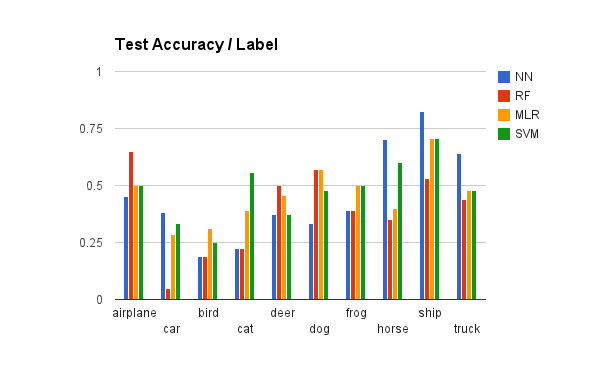
\includegraphics[width=0.5\textwidth]{pic/label_analysis.png}
    \label{label_analysis}
\end{figure}

Moreover, we compared the accuracy of classifiers label by label. To do so, we manually labeled 200 images in testing data, and calculated the accuracy of each label in different classifiers. The result is shown in Figure. \ref{label_analysis}.

We found that no classifiers dominate all label classification problems. Instead, each classifier has its strong labels and weak labels. For example, although Random Forest seemed have worst performance among 4 classifiers, but it can classify 'airplane' better than other classifiers. SVM is good at 'cat', MLR do better jobs in dog, and Neural Network is good at 'horse' and 'ship'.

The result shows that each classifier has different strong points and weak points. It indicates that if we can find a method to collaborate all classifiers, maybe the aggregated result will be better than single classifier result.

\subsection{Ensemble}

\begin{figure}[h!]
  \caption{Ensemble}
  \centering
    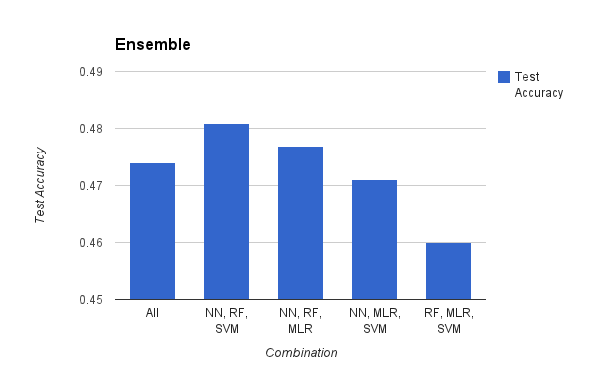
\includegraphics[width=0.5\textwidth]{pic/ensemble}
    \label{ensemble}
\end{figure}

To aggregated each classifier’s prediction, we used simple voting to combine prediction results from different classifiers, which means that the ensemble classifier will predict the most frequent predicted label of classifiers. We tried all combinations with more than 3 classifiers, and the result is show above. According to the experiment, it shows that combining predictions of Neural Network, Random Forest, and SVM has best performance. 

\begin{table}[h]
\caption{Ensemble v.s. Single Classifier}
\begin{tabular}{|c|c|c|}
\hline
 \textbf{Method}  & \textbf{Test Accuracy} & \textbf{Improvement}  \\ \hline
 NN + RF + SVM & 48.10\% & ---  \\ \hline
 NN & 47.33\% & 0.76\% \\ \hline
 SVM  & 45.85\% & 2.25\% \\ \hline
 MLR & 45.41\% & 2.69\% \\ \hline
 RF & 35.03\% & 13.07\% \\ \hline
\end{tabular}
\label{ensemble_table}
\end{table}

Comparing the ensemble method and single classifier results, shown in table \ref{ensemble_table}, the ensemble method improves accuracy about 0.76\% $\sim$ 13.07\%, which indicates that ensemble method can enhance performance of single classifier. 

\section{Conclusions}
We conducted a machine learning approach to solve multiclass image classification problem.

First, We systematically tuned four well-known machine learning algorithms: Neural Network, Random Forest, Multinomial Logistic Regression, and Support Vector Machine. We found that Neural Network has best performance in single classifier comparison.

Next, we analyzed the prediction results of four classifiers against 10 labels. We found that each classifier has its strong labels and weak labels, which indicates that ensemble method can improve performance.

Furthermore, we conducted voting ensemble method with different combinations. According to the experiment result, combining the prediction results of Neural Network, Random Forest, and Support Vector Machine enhance total performance best, which can increase accuracy 0.76\% $\sim$ 13.07\%. The result justified that voting ensemble method can help to improve performance. 


%
% The following two commands are all you need in the
% initial runs of your .tex file to
% produce the bibliography for the citations in your paper.
\bibliographystyle{abbrv}
\bibliography{sanchuah}  % sigproc.bib is the name of the Bibliography in this case
% You must have a proper ".bib" file
%  and remember to run:
% latex bibtex latex latex
% to resolve all references
%
% ACM needs 'a single self-contained file'!
%
%APPENDICES are optional
%\balancecolumns

\appendix
%Appendix A

\section{Dimension Reduction}


\begin{figure}[h!]
  \caption{Dimension Reduction}
  \centering
    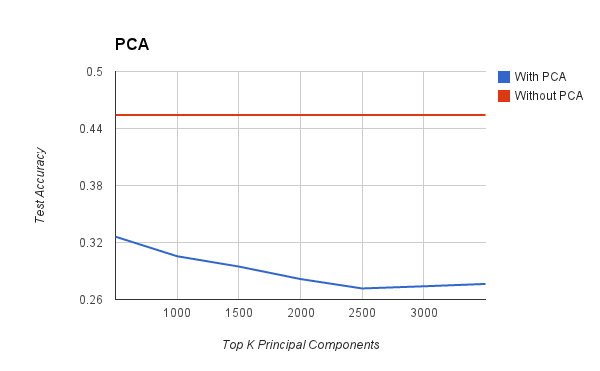
\includegraphics[width=0.5\textwidth]{pic/pca}
    \label{pca}
\end{figure}

We have tried dimension reduction with PCA, but the result showed that this method did not fit the data.

We used MLR with our basic learning algorithm, and compared the performance of the model trained on raw data, and the model trained on top-K principal components. As the result showed in Figure \ref{pca}, PCA dimension reduction decreased performance; therefore, we did not use dimension reduction with PCA in model learning process.

\section{Feature Expansion Experiment}

We compared the classifiers trained on raw data and those trained on raw data with expansion features. According the experiments, we found that feature expansion can increase accuracy of all classifiers about  0.2\% ~ 3.8\% .

The result shows that feature expansion has potential to improve performance. However, because the proposal mentioned that the image feature extraction is not the main point of this project, we did not exploit more sophisticated image features, like SIFT and GIST. Rather, we focus on utilizing different classifiers in this project.

\begin{table}[h]
\caption{Ensemble v.s. Single Classifier}
\begin{tabular}{|c|c|c|}
\hline
 \textbf{Classifier}  & \textbf{\parbox[t]{2.7cm}{Accuracy \\ without expanded features}} & \textbf{\parbox[t]{2.7cm}{Accuracy \\ with expanded features}}  \\ \hline
 NN & 43.543\% & 47.333\%  \\ \hline
 RF & 34.743\% & 35.029\% \\ \hline
 MLR  & 42.971\% & 45.410\% \\ \hline
 SVM & 42.019\% & 45.848\% \\ \hline
\end{tabular}
\label{ensemble_table}
\end{table}

\section{Division of Labor}

\textbf{SanChuan Hung (sanchuah)}
Program and tuning Kernel Multinomial Logistic Regression and SVM.
Documentation design and test result of these 2 classifiers.
Program and test feature expansion, PCA and ensemble method.
Label Analysis and result report.

\textbf{Jiajun Wang (jiajunwa)}
Learn Weka. Tuning Neural Network and Random Forest classifiers using Weka.
Documentation design and test result of these 2 classifiers.
Test ensemble method based on pre-processed data set using Neural Network and Random Forest classifiers.

\section{What we learned from project}
In this project, we tried several classifiers. Their performance is diverse. For example, although Neural Network appears to predict more accuracy than other classifiers, training and tuning it requires a lot of time and computing resource. So we have the trade-off between the tuning cost and potential accuracy when we choose the classifiers.

Then by combining different classifiers using ensemble methods, we managed to enhance the prediction accuracy. The label analysis shows that different classifiers have specify strengths on certain features/labels. So we think there should be more space for improvement. Due to the limited time and computing resource we have, we must stop at current status. If it is given more resource, we think we could using more classifiers and elaborate our ensemble method to achieve higher accuracy.

Finally, although it is not the emphasis of this project, we find feature expansion based on image processing technology do boost predication accuracy greatly. By using a relatively simple expansion strategy, we improved our test accuracy by more than 4\%. We think if we use more complicated strategy, the improvement would be more significant. However, as this is not the priority of this project, we didn't dig too deep in this direction.

\end{document}
